% Full title as you would like it to appear on the page
\chapter{Error Covariance Fitting and Optimal Telescope Control}
\label{chap:err}
\chaptermark{Error and Control}

\epigraph{By failing to prepare, you are preparing to fail.}{Benjamin Franklin}

In this chapter, we transition from developing our wavefront sensing framework to showing how it can be used to optimally control a telescope like the Rubin Observatory. The connecting bridge is the error covariance matrix of the estimated global wavefront coefficients. In Section \ref{sec:error}, we show how our framework allows this covariance to be easily computed. Then in Section \ref{sec:optcont}, we show how we can use this in control simulations and assess different control strategies.

\section{Error Covariance Fitting}
\label{sec:error}

The key breakthrough is that since the interpolation step of our algorithm has a closed form, the error covariance is a closed form function of the error covariance of our local wavefront predictions from the first step. In order to do this we first fix the positions of the 10 brightest stars on each of the four sensors. For indexing, let $(x_1,y_1)$ be the first position on the first corner sensors, $(x_{11},y_{11})$ be the first position on the second sensor, ... and $(x_{31},y_{31})$ be the first position on the fourth sensor. Then we define $\gamma$ as

\begin{equation*}
\gamma = \begin{bmatrix}
\alpha_4(x_1,y_1)\\
\dots\\
\alpha_4(x_{10}, y_{10})\\
\alpha_5(x_1,y_1)\\
\dots\\
\dots \\
\alpha_{21}(x_{10},y_{10})\\
\alpha_4(x_{11}, y_{11})\\
\dots \\
\dots \\
\alpha_4(x_{21}, y_{21})\\
\dots \\
\dots \\
\alpha_4(x_{31}, y_{31})\\
\dots \\
\dots \\
\alpha_{21}(x_{40},y_{40})\\
\end{bmatrix}
\end{equation*}

\noindent Thus $\gamma \in \mathbb{R}^{720}$, where 720 stems from 10 positions, 4 sensors, and 18 coefficients. We also make the empirically confirmed assumption that the individual local wavefront coefficient predictions are zero centered. Then the error covariance between $\gamma_1, \gamma_2$ measures the error covariance of the $\alpha_4$ predictions across donut locations on the first wavefront sensors; the error covariance between $\gamma_1, \gamma_{11}$ measures the error covariance between the $\alpha_4$ and $\alpha_5$ predictions at the same donut position; the error covariance between $\gamma_1, \gamma_{181}$ measures the error covariance of the $\alpha_4$ predictions between positions on two different corner wavefront sensors. Thus a lot of different forms of covariance are encoded in the covariance between elements of $\gamma$. The full error covariance on the local wavefront predictions is $\Sigma_{\gamma} = \text{Cov}(\gamma, \gamma)$.

We assume that the error $\gamma$ is a multi-dimensional gaussian random variable. Then the covariance from the maximum likelihood estimate is $\Sigma_{\gamma} = (X - E[X])(X-E[X])^T$ where $X \in \mathbb{R}^{497 \times 720}$ such that $X_i = \gamma^{(i)}$ the local wavefront errors from the ith observation. Figure \ref{fig:large-cov} shows the local estimate covariance matrix. 

\begin{figure}[!htbp]
\begin{center}
\begin{tabular}{c}
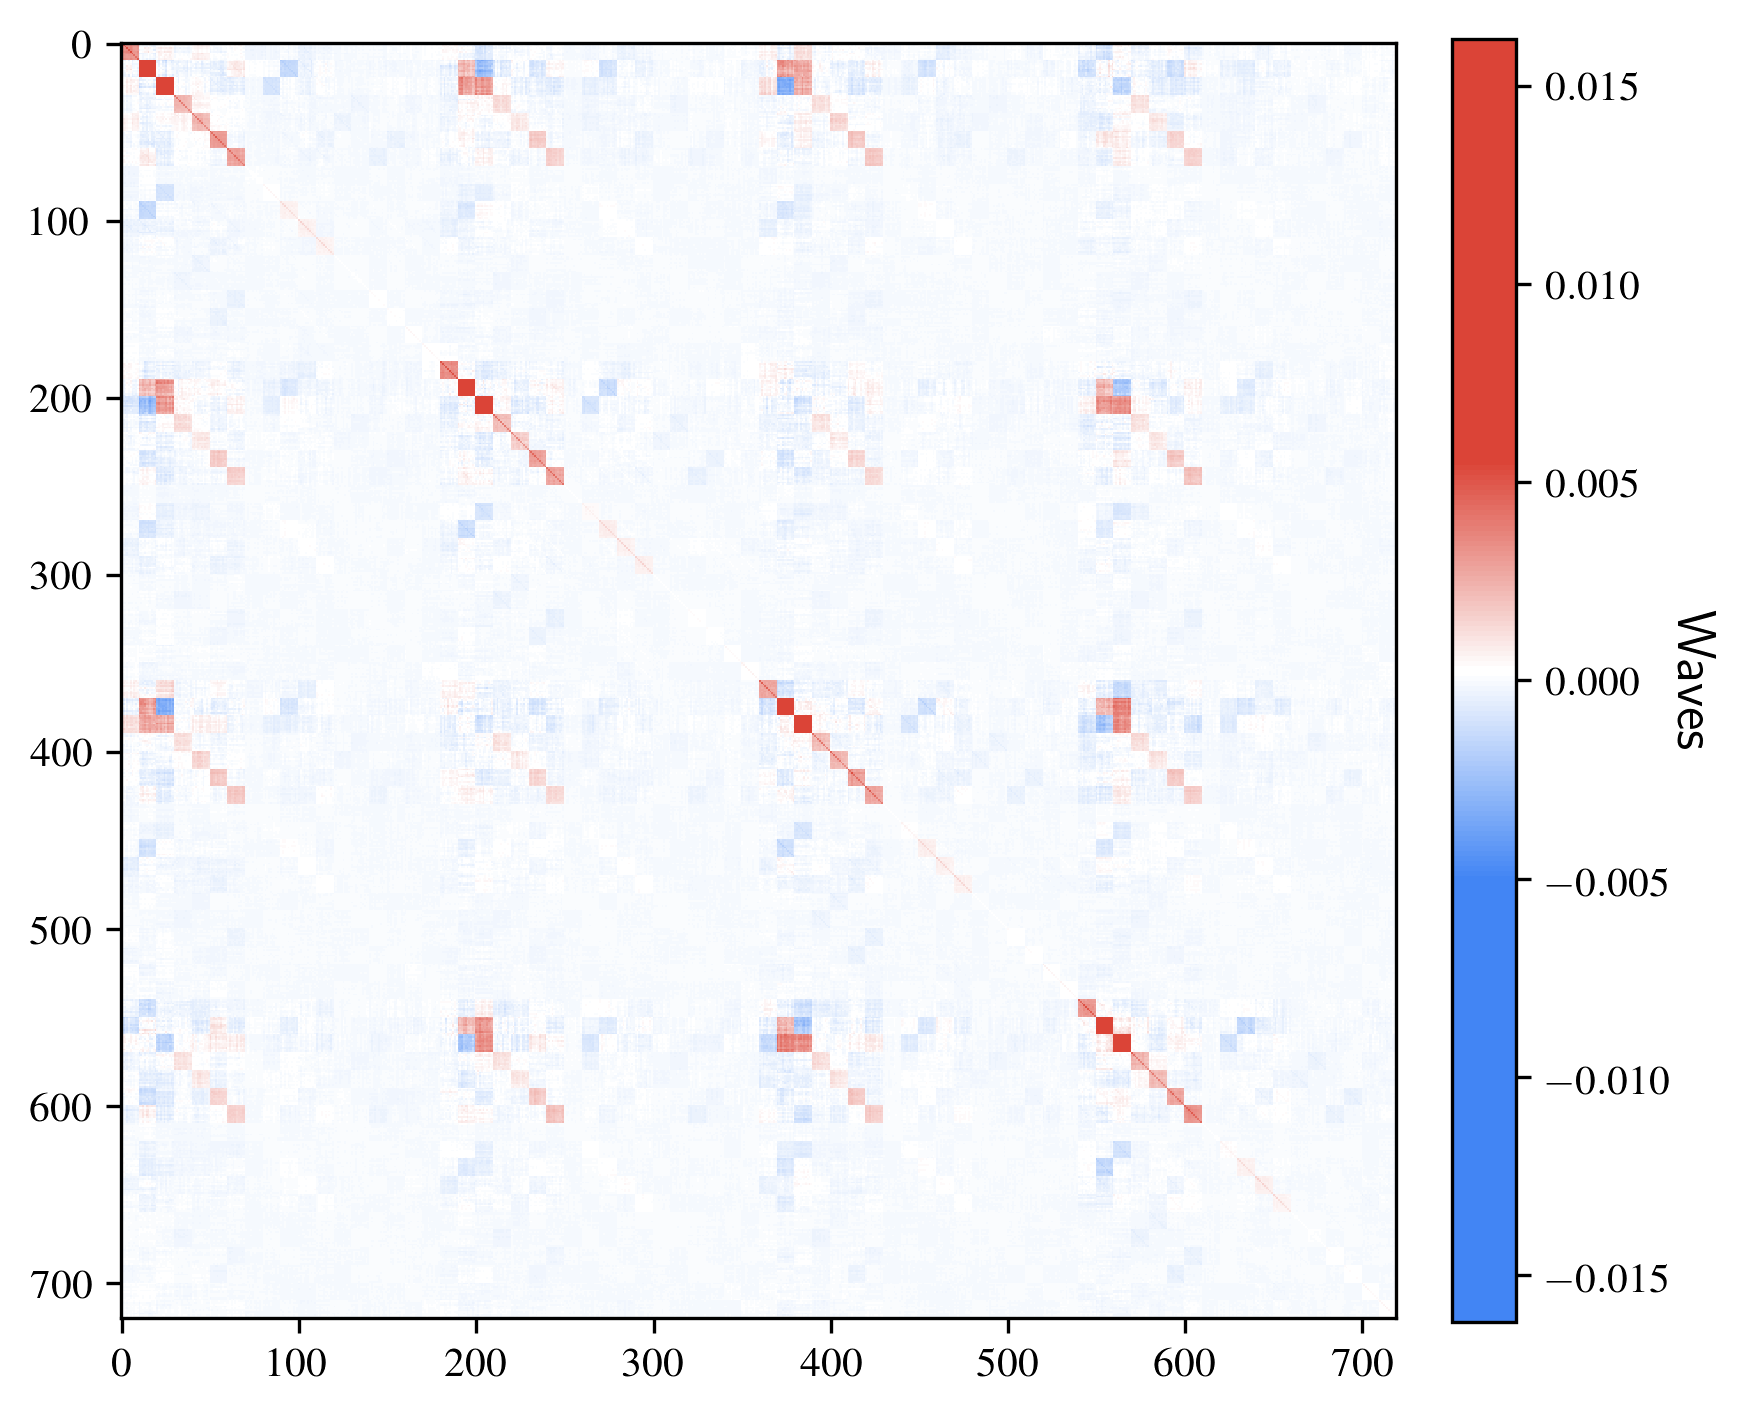
\includegraphics[width=\textwidth]{figs/control/obs_cov_written_thesis.png}
\end{tabular}
\end{center}
\caption[Error Covariance Of Local Wavefront Estimates]{The error covariance matrix $\Sigma_{\gamma}$ for the local wavefront error estimates in units of waves.\label{fig:large-cov}}
\end{figure}

Recall that if $y = Bx$, then $\text{Cov}(y,y) = B\text{Cov}(x,x)B^T$. In our case we can define an $A$, such that $\beta = (A^TA)^{-1}A^T\gamma$. This $A$ is 

\begin{equation*}
A = \begin{bmatrix}
I_{18} \otimes \begin{bmatrix}Z_1(x_1,y_1) & Z_2(x_1,y_1) & Z_3(x_1,y_1) \\ \vdots & \vdots & \vdots \\  Z_1(x_{10},y_{10}) & Z_2(x_{10},y_{10}) & Z_3(x_{10},y_{10}) \end{bmatrix}\\
I_{18} \otimes \begin{bmatrix}Z_1(x_{11},y_{11}) & Z_2(x_{11},y_{11}) & Z_3(x_{11},y_{11}) \\ \vdots & \vdots & \vdots \\  Z_1(x_{20},y_{20}) & Z_2(x_{20},y_{20}) & Z_3(x_{20},y_{20}) \end{bmatrix}\\
I_{18} \otimes \begin{bmatrix}Z_1(x_{21},y_{21}) & Z_2(x_{21},y_{21}) & Z_3(x_{21},y_{21}) \\ \vdots & \vdots & \vdots \\  Z_1(x_{30},y_{30}) & Z_2(x_{30},y_{30}) & Z_3(x_{30},y_{30}) \end{bmatrix}\\
I_{18} \otimes \begin{bmatrix}Z_1(x_{31},y_{31}) & Z_2(x_{31},y_{31}) & Z_3(x_{31},y_{31}) \\ \vdots & \vdots & \vdots \\  Z_1(x_{40},y_{40}) & Z_2(x_{40},y_{40}) & Z_3(x_{40},y_{40}) \end{bmatrix}
\end{bmatrix}
\end{equation*}

\noindent where $I_{18} \in \mathbb{R}^{18 \times 18}$ is the identity matrix, $\otimes$ is the kronecker product, and $Z_i(x_j,y_j)$ is the $jth$ circular Zernike polynomial being evaluated at focal plane position $x_j,y_j$. Then the error covariance matrix for $\beta$ is $\Sigma_{\beta} = (A^TA)^{-1}A^T\Sigma_{\gamma}A(A^TA)^{-1}$. It is shown in Figure \ref{fig:small-cov}.

\begin{figure}[!htbp]
\begin{center}
\begin{tabular}{c}
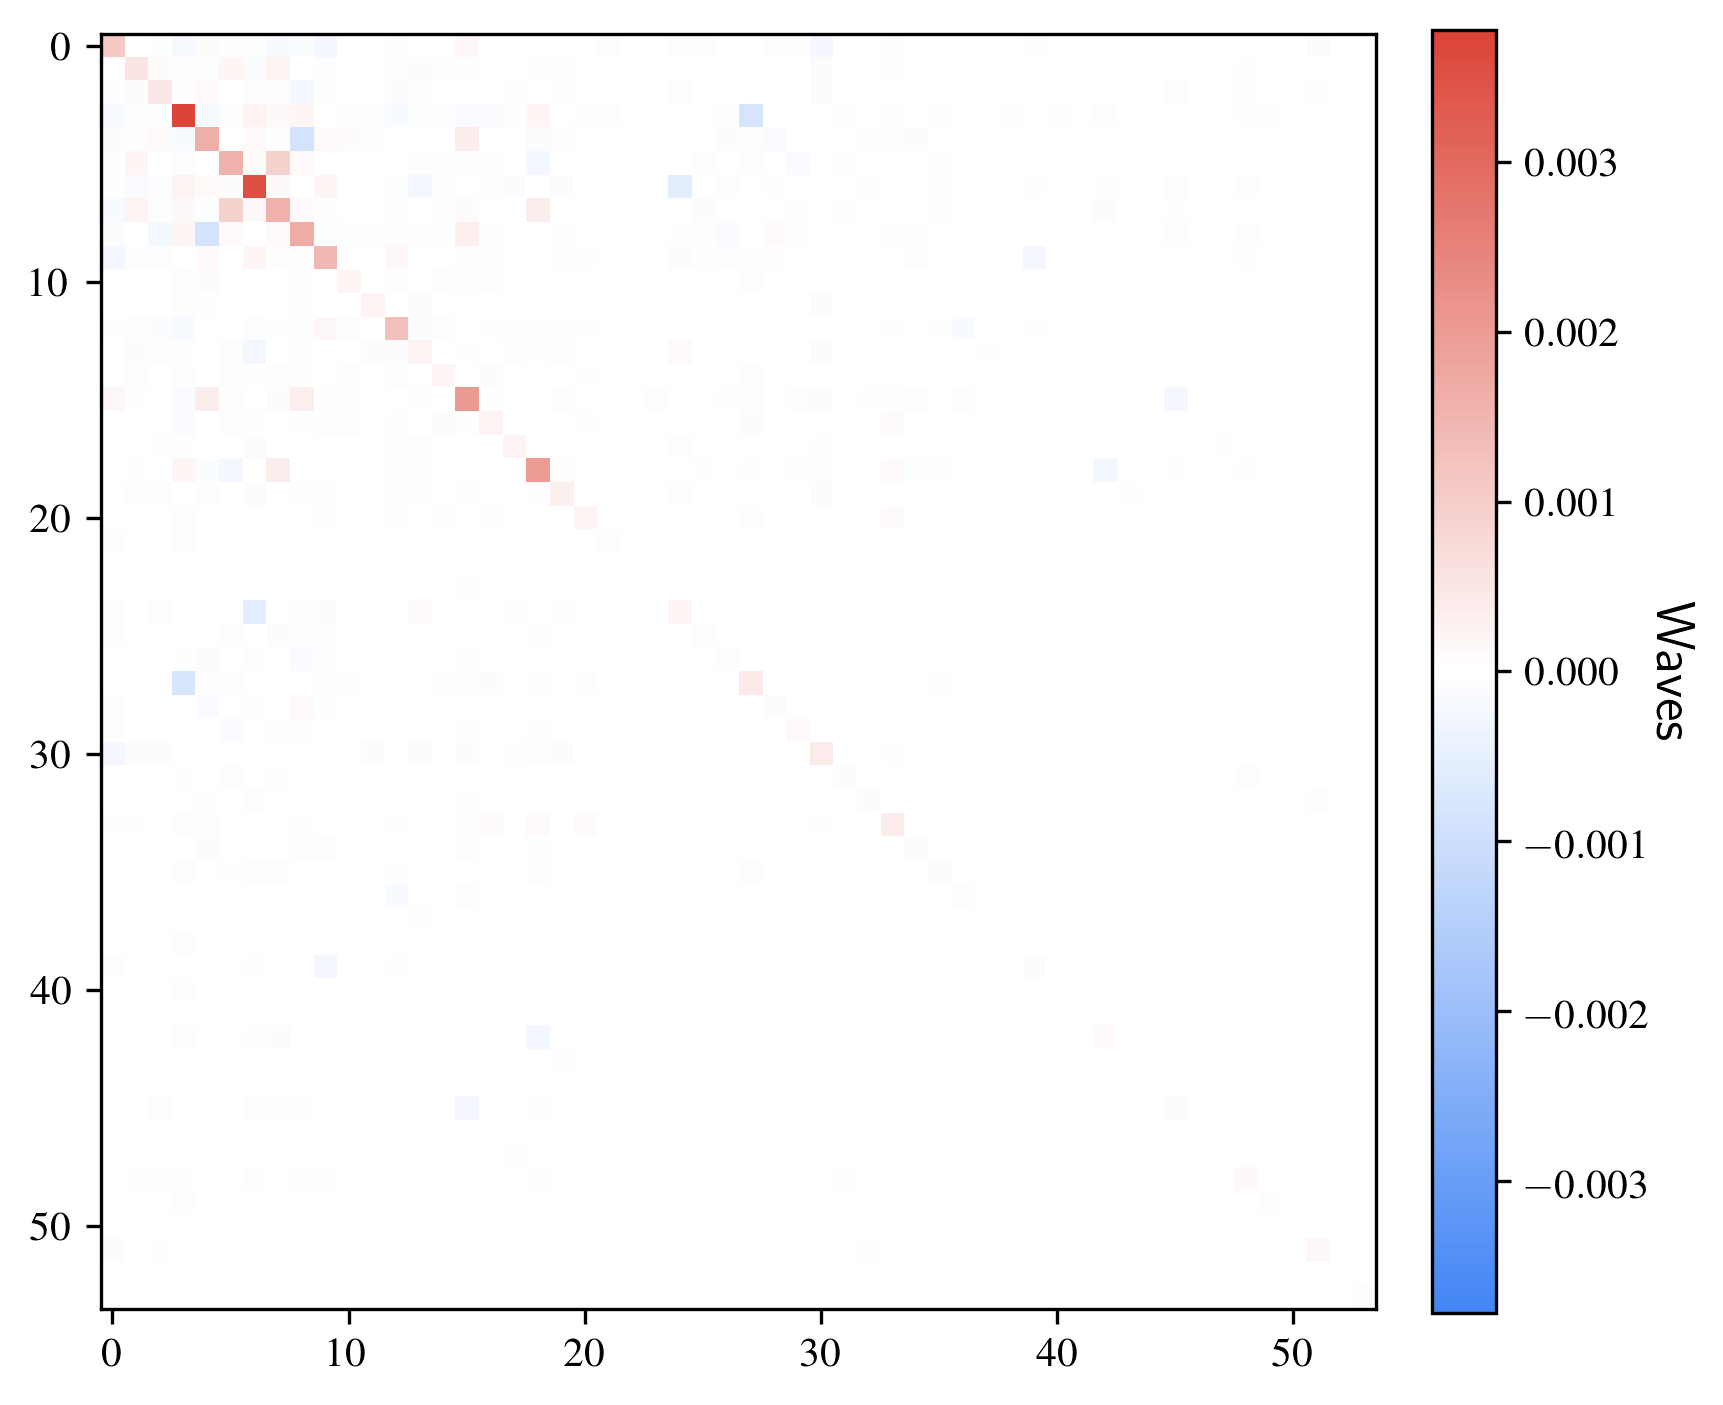
\includegraphics[width=\textwidth]{figs/control/beta_cov_written_thesis.png}
\end{tabular}
\end{center}
\caption[Error Covariance Of Global Wavefront Estimates]{The error covariance matrix $\Sigma_{\beta}$ for the global wavefront error estimates in units of waves.\label{fig:small-cov}}
\end{figure}

The global wavefront covariance $\Sigma_{\beta}$, which can be computed based on the empirically determined $\Sigma_{\gamma}$, is a key advantage to our wavefront sensing framework. We can use this statistical error model to characterize the performance of the system through time.

\section{Optimal Control}
\label{sec:optcont}

We developed a simulator in order to assess different control strategies. The simulator simulates the global wavefront coefficients over discrete time steps. There are three steps at each time step. First, a perturbation is applied. In practice, this would be caused by changes to the wind, gravitational stress, thermal gradients, etc. Second, the global wavefront prediction is made with the error covariance from the previous section. Third a control strategy is applied with this estimate. Figure \ref{fig:control-algo} summarizes the simulator algorithm. 

\begin{figure}[!htbp]
\begin{center}
\begin{tabular}{c}
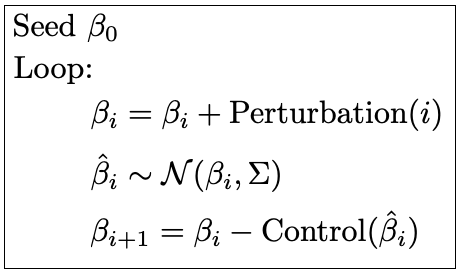
\includegraphics[width=3in]{figs/control/algo.png}
\end{tabular}
\end{center}
\caption[Control Simulator Algorithm]{The control simulator algorithm. The sequence of perturbations, error covariance matrix, and control strategy are passed by the client.\label{fig:control-algo}}
\end{figure}

We used this simulator to test four different control strategies. The first is the null control strategy which does not make any changes to the control parameters, or 

\begin{equation*}
\text{Control-Null}(\hat{\beta}_i) = \hat{\beta}_i
\end{equation*}

\noindent This is useful for null tests.

The second is a gain controller. It makes the update 
\begin{equation*}
\text{Control-Gain}(\hat{\beta}_i) = g \cdot \hat{\beta}_i
\end{equation*} 
\noindent where $g$ is the gain, which is typically less than 1. When $g=1$, this reduces to the null controller.

The third is a proportional-integral-derivative (PID) controller. It extends the gain controller with two additional additive terms. One term accumulates the estimates, the other uses the difference between the current and previous estimates as a proxy for a derivative. It makes the update

\begin{equation*}
\text{Control-PID}(\hat{\beta}_i) = c_p \cdot \hat{\beta}_i + c_i \sum_{j=1}^i \hat{\beta}_j + c_d \cdot (\hat{\beta}_i - \hat{\beta}_{i+1})
\end{equation*}

\noindent where $c_p, c_i, c_d$ are the configurable model parameters. When $c_i = c_d = 0$ it reduces to the gain controller.

The fourth is a linear-quadratic-gaussian (LQG) controller. In control theory, the separation principle says that the problem of designing an optimal controller for a stochastic system can be decomposed into (i) an optimal estimator of the state and (ii) an optimal deterministic controller. LQG adheres to this decomposition. A Kalman filter (or linear-quadratic state estimator) is used for state estimation and a linear-quadratic regulator is used for control. For our discrete time problem, the update is

\begin{align*}
\text{Control-LQC}(\hat{\beta}_i) &= K_i \cdot x_i\\
x_{i+1} &= x_i - u_i + L_i (\hat{\beta}_i - x_i + u_i)\\
x_0 &= \hat{\beta}_0\\
L_i &= P_i(P_i + \Sigma_{\beta} + V)^{-1}\\
P_{i+1} &= P_{i} - P_i (P_i + \Sigma_{\beta} + V)^{-1} P_i + V\\
P_0 &= \Sigma_{\beta} + V\\
K &= (S_h + R)^{-1} S\\
S_{i+1} &= S_i - S_i (S + R)^{-1}S + Q\\
S_0 &= Q\\
\end{align*}

\noindent where $Q,R,V$ and the horizon $h$ are configurable parameters.

In order to make the sequence of perturbations in the simulator as realistic as possible we developed code to convert contiguous observations from OpSim into sequences of perturbations. We use two types of perturbations: Jump and Box. 

Jump perturbations are applied once at a specific time step. They are parameterized by a time step and scale. The 56-dimensional global wavefront perturbation is drawn from a zero-mean multivariate normal distribuation. The covariance is $\Sigma_{\beta}$ times the scale. 

Box perturbations are parameterized by a step, duration, and scale. It begins at the step time step and lasts for the duration number of time steps. At each time step, the 56-dimensional global wavefront perturbation is drawn from a zero-mean multivariate normal distribuation. The covariance is $\Sigma_{\beta}$ times the scale. It is worth noting that for each timestep within the duration, a different perturbation is drawn and applied. Table \ref{tab:conversion} shows how we convert OpSim sequences of observations into sequences of perturbations.

\begin{table}
{
\begin{center}
\begin{tabular}{|c|c|}
\hline
Observation & Perturbation\\
\hline
First 50 Observations & Box(start=0, duration=50, scale=2)\\
Last 50 Observations & Box(start=end-50, duration=50, scale=2)\\
Slew $> 5$ & Jump(step=step, scale=5)\\
Slew $> 20$ & Jump(step=step, scale=100)\\
Filter Change & Jump(step=step, scale=20)\\
\hline
\end{tabular}
\end{center}
}
\caption[Observation To Perturbation Conversions]{The mapping between catalog observations and their corresponding perturbations for the control simulator.}
\label{tab:conversion}
\end{table}

Each of the control strategies has parameters. We randomly selected 11 nights within the 10 year observing period for Rubin. We convert each of these nights into a sequence of perturbations for the control simulator. Then we fit the control strategy parameters on the first 10 nights, and evaluate them on the held out final night. The penalty combines the norm of the state, which is zero in the nominal state, and the size of the update.

\begin{equation*}
\text{Penalty} = ||\beta_{i+1}||_2^2 + \frac{1}{2}||\text{Control}(\hat{\beta}_i)||_2^2
\end{equation*}

For the gain controller, we found a gain of 0.39 was optimal. For the PID controller, we found $c_p = 0.37, c_i= 5.4\times 10^{-06}, c_d=.15$ was optimal. For the LQG controller, we found $Q = 0.84 \cdot I_{56}, R=0.88\cdot I_{56}$ with a fixed horizon $h=5$ and $V$ equal to the covariance of the state difference between steps with the null controller on the 10 training nights. The results on the final test night are shown in Figure \ref{fig:control-results}.

\begin{figure}[!htbp]
\begin{center}
\begin{tabular}{c}
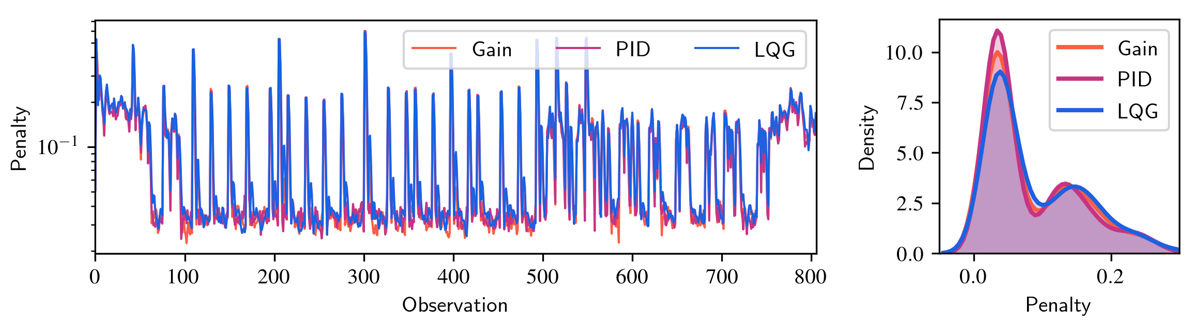
\includegraphics[width=\textwidth]{figs/control/control_results.png}
\end{tabular}
\end{center}
\caption[Controller Results]{Left: the penalty of the different controllers through time on the test night. Right: the distributions of the penalties. \label{fig:control-results}}
\end{figure}

The first thing to note is that the performance of the three non-trivial controllers is very similar. The cumulative penalty for the different methods is 1901.78, 16.22, 15.61, and 16.92 for the null, gain, PID, and LQG controllers respectively. It seems like the PID controller best balances the positives from its sophistication and parameterization with the negatives that can arise from overfitting. 

As of yet, there has not been an investigation of the tradeoffs between different control strategis for Rubin. The current plan is to spend time during commissioning to take data and develop a strategy on the mountain. However, each extra day on the mountain not only delays the survey but also runs up the project budget. The framework we have presented here
has the potential to save this critical commissioning time by enabling this work on the mountain to be done now, with this framework. 
